\clearpage
\newpage


\section{Results}\label{sec:results}
This section presents a painting placement solution to the painting placement instances in table~\ref{tab:instances}.
Obtained solutions are discussed in the following subsections –
random scenario instances in~\ref{subsec:random-scenario},
packing scenario instances in~\ref{subsec:packing-scenario},
clustering scenario instances in~\ref{subsec:clustering-scenario},
and London National Gallery instance~\ref{subsec:london-gallery-wall}.
Hyperparameter values used to obtain results in this section are in table~\ref{tab:hyperparameters-values}.
Statistics for the last iteration of the genetic algorithm for each instance are in table~\ref{tab:statistics}.

Hyperparameter values in table~\ref{tab:hyperparameters-values} are set to their recommended values
from hyperparameter testing in section~\ref{sec:hyper-parameters}.
The hyperparameter not set to the recommended values is \verb|maxNumberOfIter|.
It is set to 500 instead of a value from the recommended range \numrange{100}{150}.
The reason is to possibly find a better painting placement solution in exchange for more computation time.

The recommendation to remove orientation penalization by setting \verb|orientationWeights| to $\langle 1,1,1\rangle$ is followed.
As described in hyperparameter testing, it should produce a population with a better on-average objective value and a faster-decreasing trend in objective value.
Also, the population size is set to 75 times the instance size.
It is the midpoint of the recommended interval \numrange{50}{100}.
Lastly, population division is set to the same values as in listing~\ref{lst:computation-submission-dataset}.
It means keeping an elitism strategy and injecting random individuals.


\begin{table}[h!]
    \caption{Hyperparameter values used to obtain results}
    \label{tab:hyperparameters-values}
    \begin{threeparttable}
        \begin{tabular}{ll}
            \hline
            \textbf{Hyperparameter}                           & \textbf{Value}             \\ \hline
            \verb|maxNumberOfIter|                            & 500                        \\ \hline
            \verb|populationSize|                             & 75 times the instance size \\ \hline
            \verb|maximumWildCardCount|                       & 1                          \\ \hline
            \verb|orientationWeights|                         & $\langle 1,1,1 \rangle$    \\ \hline
            \verb|populationDivisionCounts|                   & elitism, random            \\ \hline
            \verb|initialPopulationDivisionCounts|            & 0.7 random, 0.3 greedy     \\ \hline
            \verb|overlappingPenalizationConstant| & \begin{tabular}[c]{@{}l@{}}
                                                         4 times the diagonal length\\ of the layout
            \end{tabular} \\ \hline
            \verb|outsideOfAllocatedAreaPenalizationConstant| & 0                          \\ \hline
        \end{tabular}
        \begin{tablenotes}
            \small
            \item Hyperparameter description is in table~\ref{tab:hyperparameters-description}.
        \end{tablenotes}
    \end{threeparttable}
\end{table}

\begin{table}[h!]
    \caption{Statistics of the last iteration}
    \label{tab:statistics}
    \begin{threeparttable}
        \begin{tabular}{lllll}
            \hline
            \textbf{Instance name} &
            \textbf{\begin{tabular}[c]{@{}l@{}}
                        Best obj.\\ value
            \end{tabular}} &
            \textbf{\begin{tabular}[c]{@{}l@{}}
                        Worst obj.\\ value
            \end{tabular}} &
            \textbf{\begin{tabular}[c]{@{}l@{}}
                        Obj.\\ mean
            \end{tabular}} &
            \textbf{\begin{tabular}[c]{@{}l@{}}
                        Standard\\ deviation
            \end{tabular}} \\ \hline
            random\_10            & 1136.11 & 3438.01  & 1640.91 & 460.76  \\ \hline
            random\_20            & 5417.8  & 11629.59 & 7209.22 & 1400.13 \\ \hline
            packing\_10           & 669.48  & 2369.11  & 1142.96 & 383.22  \\ \hline
            packing\_20           & 6219.13 & 12283.41 & 8140.29 & 1450.09 \\ \hline
            cluster\_3\_6         & 3921.68 & 11121.96 & 6317.36 & 1844.99 \\ \hline
            cluster\_4\_5         & 4887.04 & 12088.99 & 7177.9  & 1767.67 \\ \hline
            london\_gallery\_wall & 2759.65 & 15764.31 & 5440.9  & 2633.81 \\ \hline
        \end{tabular}
        \begin{tablenotes}
            \small
            \item Instance description is in table~\ref{tab:instances}.
        \end{tablenotes}
    \end{threeparttable}
\end{table}

\newpage

\subsection{Random scenario}\label{subsec:random-scenario}

Visualization of the painting placement solution to the random\_10 instance
is in figure~\ref{fig:results:visualization-random-10}
and for random\_20 instance in figure~\ref{fig:results:visualization-random-20}.

For the random\_10 instance, we can see that there are no overlappings, and only painting~6 is partially outside the layout.
Also, due to the eval function set to $f(x,y) = x+y$, smaller paintings
are placed towards the bottom left corner.
This painting placement solution can be considered successful,
because it adheres to all penalizations that are applied.

For the random\_20 instance, we can see that there are four overlappings.
Similarly to the random\_10 instance, the eval function forced the placement of the
smaller paintings to the bottom left corner, and one painting is placed outside the layout.
Due to the four overlappings, it is only a partially successful painting placement solution.
On the other hand, the solution adheres to all other penalizations.
It might suggest further increasing the overlapping penalization constant~$\lambda$.

\subsection{Packing scenario}\label{subsec:packing-scenario}
Visualization of the painting placement solution to the packing\_10 instance
is in figure~\ref{fig:results:visualization-packing-10}
and for packing\_20 instance in figure~\ref{fig:results:visualization-packing-20}.

For the packing\_10 instance, we can see no overlappings, and paintings~2,3,4 are partially outside the layout.
It is considered a success, as the packing scenario tests the ability to form compact solutions by setting the instance generation parameter
layout area ratio to one, which means that the area of the layout equals the area of all paintings summed together.
However, an improvement in compactness can still be gained by moving paintings 1 and 2 downwards.
It could be implemented using a post-optimization, suggested in subsection~\ref{subsec:post-optimization}.
The eval function is absent in the packing scenario, so there is no preference for any part of the layout.

For the packing\_20 instance, we can see seven overlapping pairs.
It is not considered a success as there is no eval function present and overlapping penalization constant~$\lambda$
should be the main source of improvement in the objective function~\ref{eq:objective}.
However, the packing complexity for 20 paintings is high, and it might be impossible to fit all paintings to the layout without overlapping or being outside the allocated area.
Also, randomly generated flow between paintings might play a role.
Nevertheless, the suggestion is to increase the overlapping penalization constant~$\lambda$.

\subsection{Clustering scenario}\label{subsec:clustering-scenario}

Visualization of the painting placement solution to the cluster\_3\_6 instance
is in figure~\ref{fig:results:visualization-cluster-3-6}
and for cluster\_4\_5 instance in figure~\ref{fig:results:visualization-cluster-4-5}.

For cluster\_3\_6 instance, we can see the formation of clusters.
It is a success as the proposed solution can recognize
the information encoded in the flow between paintings.
However, we can see that there are seven overlappings.
An interesting fact is that these overlappings are only inside the same clusters.
It suggests that the flow between paintings is set too high,
so it is advantageous to create overlaps and thus decrease the flow.

For the cluster\_4\_5 instance, we can see a partially successful formation of clusters.
It still suffers from the problems of overlapping paintings in the same cluster.
However, there are also several overlappings between paintings from different clusters.
It might suggest that the overlapping penalization and flow are more balanced.

\subsection{London Gallery Wall}\label{subsec:london-gallery-wall}

Visualization of the painting placement solution to the london\_gallery\_wall instance
is in figure~\ref{fig:results:visualization-london-gallery-wall}.
The instance is created from the painting placement at the London National Gallery from figure~\ref{fig:london-wall}.
Also, the flow between paintings is set to reassemble the relative positions from that figure
(concrete flow values are in the dataset in the attached medium).

We can see that the obtained solution contains no overlappings, and two paintings are partially placed outside the layout.
Also, most of the relative positions of the paintings are successfully reconstructed using the flow.
The difference is that the proposed solution placed the largest middle painting to the right of the layout
instead of in the middle, as seen in the original figure.
However, the flow can be changed to obtain different results.


\clearpage
\newpage

\begin{figure}[h!]
    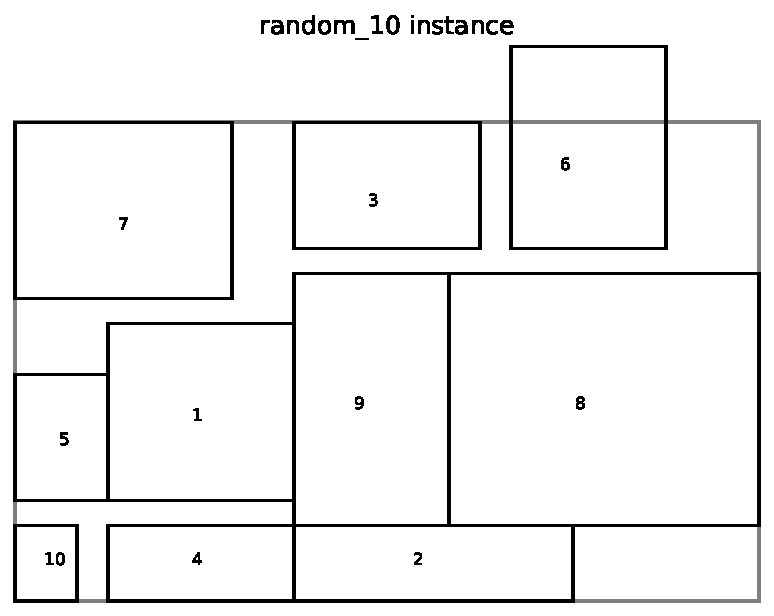
\includegraphics[width=0.8\textwidth, center]{visualizations/visualization_random_10}
    \caption[Painting placement solution for the random\_10 instance]
        {Painting placement solution for the random\_10 instance.
    There are no overlappings.}
    \label{fig:results:visualization-random-10}
\end{figure}

\begin{figure}[h!]
    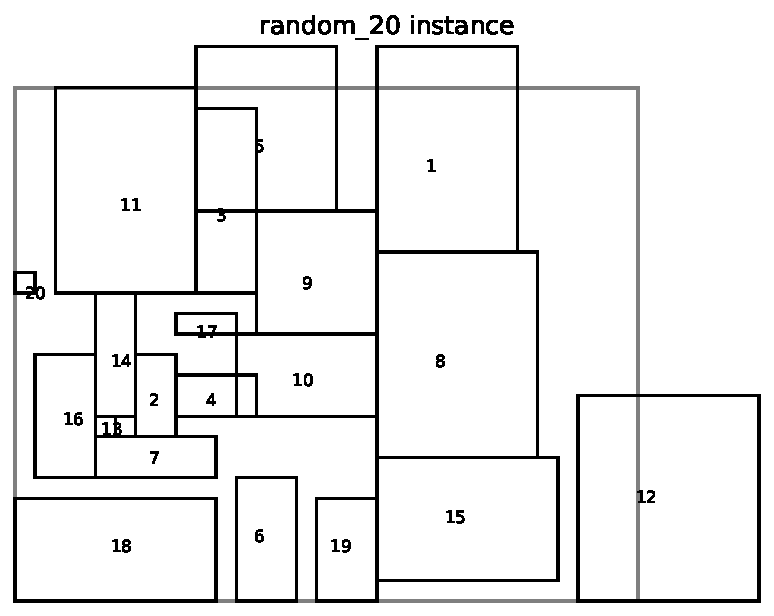
\includegraphics[width=0.8\textwidth, center]{visualizations/visualization_random_20}
    \caption[Painting placement solution for the random\_20 instance]
        {Painting placement solution for the random\_20 instance.
    Four overlapping pairs exist (15–18, 15–16, 3–10, 9–11).}
    \label{fig:results:visualization-random-20}
\end{figure}

\begin{figure}[h!]
    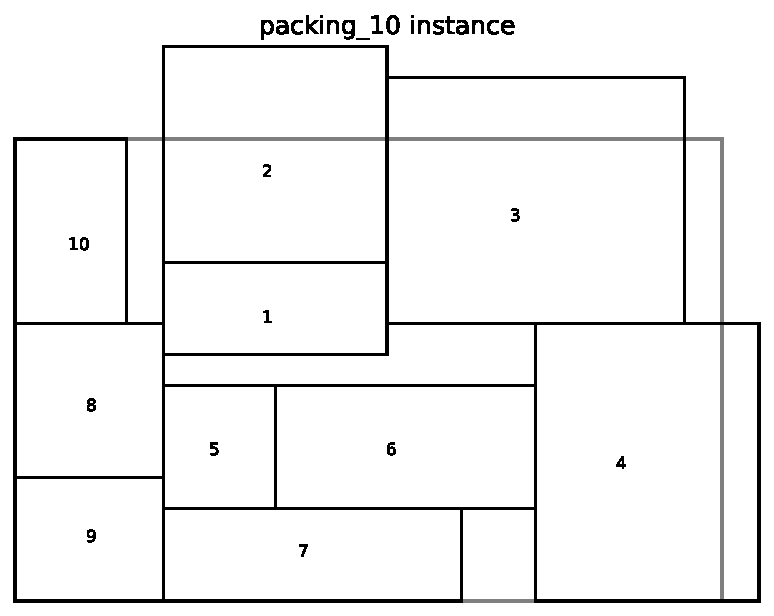
\includegraphics[width=0.8\textwidth, center]{visualizations/visualization_packing_10}
    \caption[Painting placement solution for the packing\_10 instance]
        {Painting placement solution for the packing\_10 instance.
    There are no overlappings.}
    \label{fig:results:visualization-packing-10}
\end{figure}

\begin{figure}[h!]
    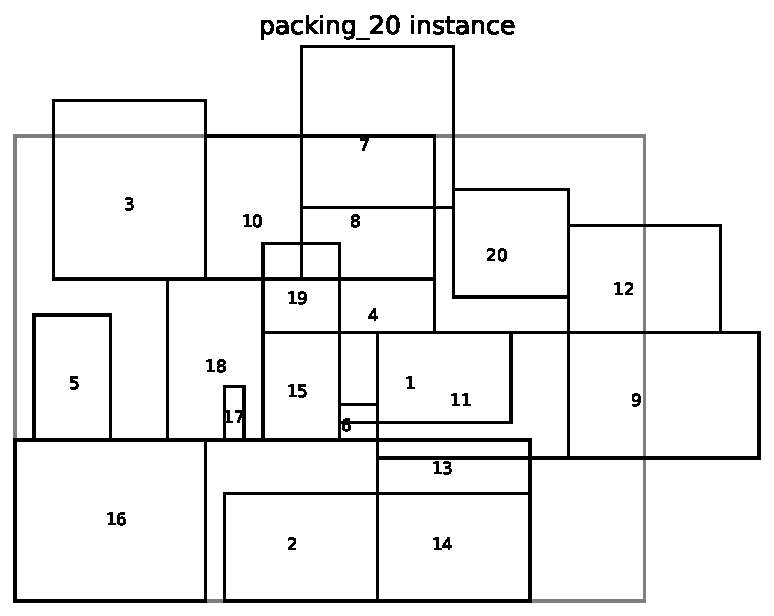
\includegraphics[width=0.8\textwidth, center]{visualizations/visualization_packing_20}
    \caption[Painting placement solution for the packing\_20 instance]
        {Painting placement solution for the packing\_20 instance.
    There are seven overlapping pairs (17–18, 1–6, 1–11, 11–13, 10–19, 8–19, 7–8).}
    \label{fig:results:visualization-packing-20}
\end{figure}

\begin{figure}[h!]
    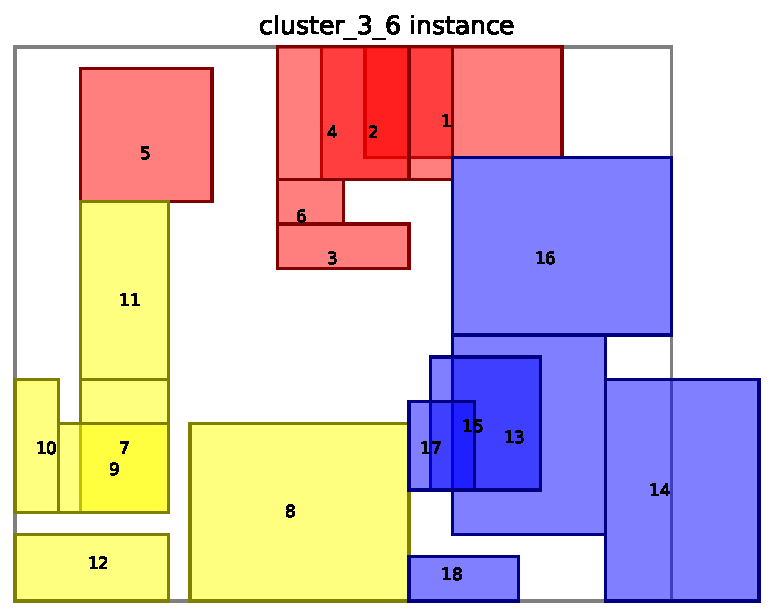
\includegraphics[width=0.8\textwidth, center]{visualizations/visualization_cluster_3_6}
    \caption[Painting placement solution for the cluster\_3\_6 instance]
        { Painting placement solution for the cluster\_3\_6 instance.
    Three groups of paintings, \numrange{1}{6}, \numrange{7}{12}, and \numrange{13}{18}, are marked using different colors.
    There are seven overlapping pairs.}
    \label{fig:results:visualization-cluster-3-6}
\end{figure}

\begin{figure}[h!]
    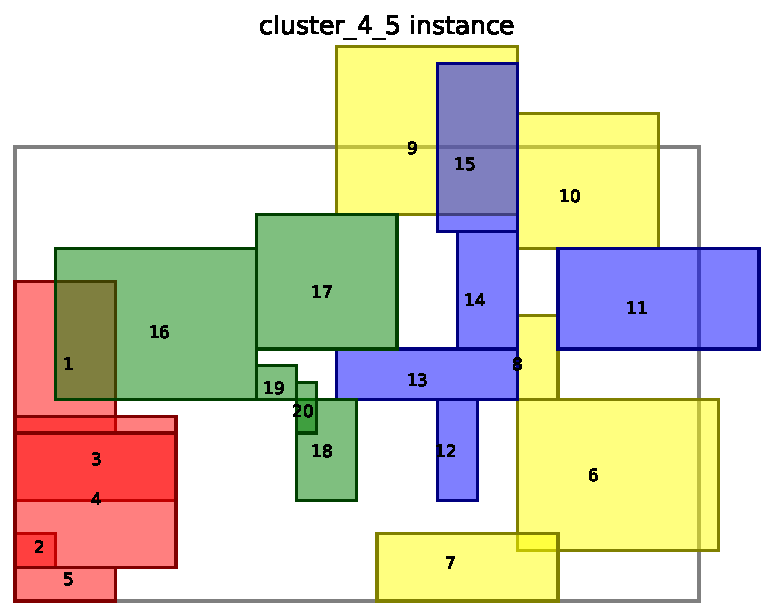
\includegraphics[width=0.8\textwidth, center]{visualizations/visualization_cluster_4_5}
    \caption[Painting placement solution for the cluster\_4\_5 instance]
        { Painting placement solution for the cluster\_4\_5 instance.
    Four groups of paintings, \numrange{1}{5}, \numrange{6}{10}, \numrange{11}{15}, and \numrange{15}{20}, are marked using different colors.
    There are seven overlapping pairs.}
    \label{fig:results:visualization-cluster-4-5}
\end{figure}

\begin{figure}[h!]
    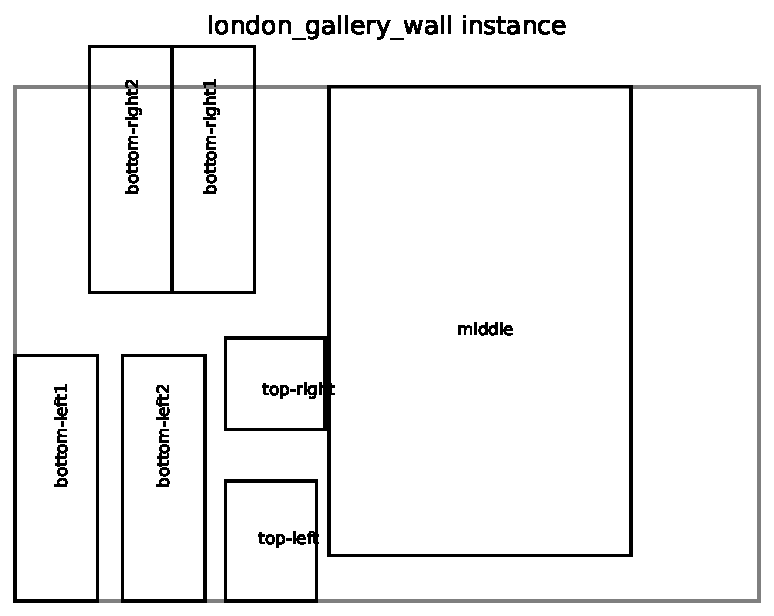
\includegraphics[width=0.8\textwidth, center]{visualizations/visualization_london_gallery_wall}
    \caption[Painting placement solution for the london\_gallery\_wall instance]
        { Painting placement solution for the london\_gallery\_wall instance.
    Paintings are marked using their original position in figure~\ref{fig:london-wall}.
    There are no overlappings.}
    \label{fig:results:visualization-london-gallery-wall}
\end{figure}
